% Options for packages loaded elsewhere
\PassOptionsToPackage{unicode}{hyperref}
\PassOptionsToPackage{hyphens}{url}
%
\documentclass[
  12pt,
]{article}
\usepackage{amsmath,amssymb}
\usepackage{lmodern}
\usepackage{iftex}
\ifPDFTeX
  \usepackage[T1]{fontenc}
  \usepackage[utf8]{inputenc}
  \usepackage{textcomp} % provide euro and other symbols
\else % if luatex or xetex
  \usepackage{unicode-math}
  \defaultfontfeatures{Scale=MatchLowercase}
  \defaultfontfeatures[\rmfamily]{Ligatures=TeX,Scale=1}
  \setmainfont[]{Times New Roman}
\fi
% Use upquote if available, for straight quotes in verbatim environments
\IfFileExists{upquote.sty}{\usepackage{upquote}}{}
\IfFileExists{microtype.sty}{% use microtype if available
  \usepackage[]{microtype}
  \UseMicrotypeSet[protrusion]{basicmath} % disable protrusion for tt fonts
}{}
\makeatletter
\@ifundefined{KOMAClassName}{% if non-KOMA class
  \IfFileExists{parskip.sty}{%
    \usepackage{parskip}
  }{% else
    \setlength{\parindent}{0pt}
    \setlength{\parskip}{6pt plus 2pt minus 1pt}}
}{% if KOMA class
  \KOMAoptions{parskip=half}}
\makeatother
\usepackage{xcolor}
\usepackage[margin=2.54cm]{geometry}
\usepackage{longtable,booktabs,array}
\usepackage{calc} % for calculating minipage widths
% Correct order of tables after \paragraph or \subparagraph
\usepackage{etoolbox}
\makeatletter
\patchcmd\longtable{\par}{\if@noskipsec\mbox{}\fi\par}{}{}
\makeatother
% Allow footnotes in longtable head/foot
\IfFileExists{footnotehyper.sty}{\usepackage{footnotehyper}}{\usepackage{footnote}}
\makesavenoteenv{longtable}
\usepackage{graphicx}
\makeatletter
\def\maxwidth{\ifdim\Gin@nat@width>\linewidth\linewidth\else\Gin@nat@width\fi}
\def\maxheight{\ifdim\Gin@nat@height>\textheight\textheight\else\Gin@nat@height\fi}
\makeatother
% Scale images if necessary, so that they will not overflow the page
% margins by default, and it is still possible to overwrite the defaults
% using explicit options in \includegraphics[width, height, ...]{}
\setkeys{Gin}{width=\maxwidth,height=\maxheight,keepaspectratio}
% Set default figure placement to htbp
\makeatletter
\def\fps@figure{htbp}
\makeatother
\setlength{\emergencystretch}{3em} % prevent overfull lines
\providecommand{\tightlist}{%
  \setlength{\itemsep}{0pt}\setlength{\parskip}{0pt}}
\setcounter{secnumdepth}{5}
\ifLuaTeX
  \usepackage{selnolig}  % disable illegal ligatures
\fi
\IfFileExists{bookmark.sty}{\usepackage{bookmark}}{\usepackage{hyperref}}
\IfFileExists{xurl.sty}{\usepackage{xurl}}{} % add URL line breaks if available
\urlstyle{same} % disable monospaced font for URLs
\hypersetup{
  pdftitle={California's Motor Vehicle Registration Fee Program's impact on the state's emission},
  pdfauthor={Shidi Dai, Soumya Mathew, Yuxuan Tian},
  hidelinks,
  pdfcreator={LaTeX via pandoc}}

\title{California's Motor Vehicle Registration Fee Program's impact on
the state's emission}
\usepackage{etoolbox}
\makeatletter
\providecommand{\subtitle}[1]{% add subtitle to \maketitle
  \apptocmd{\@title}{\par {\large #1 \par}}{}{}
}
\makeatother
\subtitle{\url{https://github.com/tyx1719/Final-Project_Shidi-Soumya-Yuxuan.git}}
\author{Shidi Dai, Soumya Mathew, Yuxuan Tian}
\date{}

\begin{document}
\maketitle

\newpage
\tableofcontents 
\newpage
\listoftables

Table 1. Dataset Description Table \newpage

\listoffigures

\emph{Figure 1.} Change in the variety of vehicles across time
\emph{Figure 2.} Change in the gasoline vehicles across time
\emph{Figure 3.} Change in share of heavy duty vehicles across time
\emph{Figure 4.} Change in share of light duty vehicles across time
\emph{Figure 5.} Trend of Nitrogen Oxide emission of diesel run vehicles
across time \emph{Figure 6.} Trend of Carbon Monoxide emission of diesel
run vehicles across time \emph{Figure 7.} Trend of Nitrogen Oxide
emission of gas run vehicles across time \emph{Figure 8.} Trend of
Carbon Monoxide emission of gas run vehicles across time \emph{Figure
9.} Trend of Nitrogen Oxide emission of light−duty vehicles across time
\emph{Figure 10.} Trend of Carbon Monoxide emission of light duty
vehicles across time \emph{Figure 11.} Trend of Nitrogen Oxide emission
of heavy−duty vehicles across time \emph{Figure 12.} Trend of Carbon
Monoxide emission of heavy duty vehicles across time \newpage

\hypertarget{project-set-up}{%
\section{Project set up}\label{project-set-up}}

\hypertarget{rationale-and-research-questions}{%
\section{Rationale and Research
Questions}\label{rationale-and-research-questions}}

\hypertarget{rationale-for-the-study}{%
\subsection{Rationale for the study}\label{rationale-for-the-study}}

This study examines the number and types of on road motor vehicles that
are most responsible for California's carbon monoxide and nitrogen oxide
emissions over the course of 5 years (2018--2022).\\
Despite an increase in population and automobile use, aggressive air
pollution control measures in California have resulted in ongoing
improvements in air quality. The state still lags the rest of the
country, even though the situation has been gradually getting better.
The state of California continues to experience worsening smog due to
its population growth, reliance on automobile travel, and warm climate.
The Advanced Clean Cars II rule, which was approved by the California
Air Resources Board in August 2022, will put California on a path to
rapidly expanding the market for zero-emission cars, pickup trucks, and
SUVs by 2035 while also bringing about cleaner air and significant
reductions in pollution that contributes to global warming{[}1{]}. The
2022 scoping plan, a five-year climate change strategy, details
California's intention to reduce its dependency on oil while also
cleaning up the worst air pollution in the country{[}2{]}. The plan also
establishes a more aggressive target of reducing carbon emissions by
48\% below 1990 levels by 2030, as opposed to the 40\% reduction by 2030
mandated by state law. To reach the new 48\% objective in just eight
years, California, however, still has a long way to go. The reduction in
emissions from 1990 levels by 2020 was just about 14\% {[}3{]}.
Furthermore, California is second among US states in terms of overall
yearly CO2 emissions of 358.6 million metric tons (Texas ranked first at
706.5 million metric ton emissions){[}4{]}. Given the strict legislation
to control emissions and the present gap between released and planned
emissions, California state is a good case study to understand the
patterns of emissions and the types of vehicles responsible for maximum
contribution.

\hypertarget{rationale-for-your-choice-of-dataset}{%
\subsection{Rationale for your choice of
dataset}\label{rationale-for-your-choice-of-dataset}}

Data from the California Department of Motor Vehicles and the California
Air Resources Board are used in this research. As the research studies
the trends of the number of vehicles in the state which likely impacts
emissions, the motor vehicle data set is useful as it provides total
vehicle counts for registered cars with precise as of dates, broken down
by ZIP code, model year, fuel type, make, and duty (light/heavy). The
study also examines how the total number of different types of vehicles
impacts the state's emissions. The emission data is useful to examine
the relationship between the type and quantity of vehicles on state's
emissions as it provides annual averages of carbon monoxide and nitrogen
oxide emitted by different subcategories of on-road motor vehicles.

\newpage

\hypertarget{dataset-information}{%
\section{Dataset Information}\label{dataset-information}}

This project uses data from two sources: California Air Resources Board
(CARB) and California Department of Motor Vehicles (CADMV). Both
datasets were retrieved on November 23, 2022.

For the emissions data, the project group uses California Air Resources
Board's Standard Emission Tool to gather statewide annual average
emissions from mobile sources from 2018 to 2022. Since the most
emissions from mobile sources are carbon monoxide and nitrogen oxides,
this project focuses on the emissions data of these two pollutants.
Therefore, there are two data files, one for carbon monoxide and the
other for nitrogen oxides. Both datasets contain emissions from 2018 to
2022 under two main mobile categories: on-road motor vehicles and other
mobile sources. Under on-road motor vehicles, there are 21
subcategories. From the websites' variable descriptions, all
subcategories with ``heavy duty'' in their names are considered heavy
duty motor vehicles, others are considered as light duty vehicles. Also,
all categories listed ``diesel'' are diesel-fueled, others are
gas-fueled.

Correspondingly, this project uses vehicle number by fuel type data from
California Department of Motor Vehicles from 2018 to 2022, to compare
with emissions data for the analyses. This includes four reports that
provide vehicle counts broken down by Zip code, model year, fuel type,
make, and duty of registered vehicles. As the 2018 report was collected
on October 1, 2018, while all other reports were collected on January 1
of 2020, 2021, and 2022, and there was no report in 2019, this project
uses the 2018 report for both 2018 and 2019 vehicle count data. In each
report, it provides vehicle counts in the last column for different
groups of year, fuel, make, and duty registered in different locations.

Limitations: Since the emissions data is annual average, there are few
observations for us to analyze. Due to the unmatched categories of
quantity and emission data, we are not able to conduct a more detailed
analysis. Also, the regression result is restricted to the limited
availability of the data. With a larger and more detailed dataset, the
result of the regression could be more robust.

\hypertarget{data-wrangling}{%
\subsection{Data Wrangling}\label{data-wrangling}}

The project group processed raw datasets from both sources for analysis
purposes.

For the vehicle counts by fuel type data from California Department of
Motor Vehicles, we wrangled the datasets to show the number of vehicles
registered in California with different fuel types. Using the unique
function, we found that there are 9 types of fuels: gasoline, diesel and
diesel hybrid, natural gas, hybrid gasoline, flex-fuel, battery
electric, other, plug-in hybrid, and hydrogen fuel cell. Thus, we summed
the number of vehicles in the vehicle column conditioned to each fuel
type in all four data sets and created a new dataframe
``VehicleNumber.Fuel'' containing information about number of vehicles
registered using different fuels in year 2018 to 2022. We converted
characters in this dataframe into numeric for later analyses use. Then
we saved this processed data set into the processed folder.

From the vehicle counts raw datasets, there is one column named ``Duty''
which differentiates vehicles with either ``light'' or ``heavy''. As
this project will be analyzing the effects of heavy and light (gasoline
and diesel) vehicles on carbon monoxide and nitrogen oxides emissions,
we summed the number of vehicles in rows with two conditions: duty and
fuel. We created new dataframes: GasolineVehicle.Duty and
DieselVehicle.Duty. In the GasolineVehicle.Duty dataset, we sum the
number of vehicles with heavy in Duty and gasoline in the fuel column,
and light in Duty and gasoline in Fuel, in years 2018 to 2022. In the
DieselVehicle.Duty dataset, we sum the number of vehicles with heavy in
Duty and diesel and diesel hybrid in Fuel, and light in Duty and diesel
and diesel hybrid in Fuel. We did similar steps to create new datasets
for heavy and light vehicle numbers using hybrid gasoline, natural gas,
and flex-fuel. Finally, we used rbind and mutate to combine all the
previous datasets into a new dataset ``Master\_table\_vehicles'', with
year, number of heavy vehicles, number of light vehicles, fuel type,
total number of vehicles, share of light vehicles in total vehicles, and
share of heavy vehicles in total vehicles. Notably, we added the two
percentage columns at the end to represent the share of light/heavy
vehicles among all. Then, we saved this dataframe in the processed data.

The project group then wrangled the two emissions datasets. As this
project is focused on motor vehicles, we only need emissions data from
on-road motor vehicles. Thus, we select only on-road motor vehicles data
from both datasets. We found that it would be easier for regression
purposes to have categories as column names and years as row names, so
we reformatted the datasets to change the rows and columns. Then, we
saved the two new dataframes as ``COT'' and ``NOX'' in the processed
folder.

We also created some more dataframes from those two datasets. We pulled
out columns with diesel vehicles to form COT.diesel and NOX.diesel.
Similarly, we pulled out columns with gasoline fueled vehicles to form
COT.gas and NOX.gas. We also pulled out columns with light duty vehicles
to form COT.light and NOX.light. We selected columns with heavy duty
vehicles to form COT.heavy and NOX.heavy. Then, we changed all the
characters to numeric form for calculation use.

\hypertarget{dataset-description-table}{%
\subsubsection{Dataset Description
Table}\label{dataset-description-table}}

\begin{longtable}[]{@{}
  >{\raggedright\arraybackslash}p{(\columnwidth - 8\tabcolsep) * \real{0.1828}}
  >{\raggedright\arraybackslash}p{(\columnwidth - 8\tabcolsep) * \real{0.2043}}
  >{\raggedright\arraybackslash}p{(\columnwidth - 8\tabcolsep) * \real{0.2043}}
  >{\raggedright\arraybackslash}p{(\columnwidth - 8\tabcolsep) * \real{0.2043}}
  >{\raggedright\arraybackslash}p{(\columnwidth - 8\tabcolsep) * \real{0.2043}}@{}}
\toprule()
\begin{minipage}[b]{\linewidth}\raggedright
Description\_Name
\end{minipage} & \begin{minipage}[b]{\linewidth}\raggedright
Vehicle.Count.2018
\end{minipage} & \begin{minipage}[b]{\linewidth}\raggedright
Vehicle.Count.2020
\end{minipage} & \begin{minipage}[b]{\linewidth}\raggedright
Vehicle.Count.2021
\end{minipage} & \begin{minipage}[b]{\linewidth}\raggedright
Vehicle.Count.2022
\end{minipage} \\
\midrule()
\endhead
\# of Variables & 7 & 7 & 7 & 7 \\
Variable Tested & Vehicles & Vehicles & Vehicles & Vehicles \\
Unit & Vehicle & Vehicle & Vehicle & Vehicle \\
Time Range & 2018 & 2020 & 2021 & 2022 \\
Observation & 586233 & 602394 & 677969 & 722465 \\
Raw/Processed & Raw & Raw & Raw & Raw \\
Class & Factor & Factor & Factor & Factor \\
Source & CADMV & CADMV & CADMV & CADMV \\
\bottomrule()
\end{longtable}

\begin{longtable}[]{@{}
  >{\raggedright\arraybackslash}p{(\columnwidth - 10\tabcolsep) * \real{0.1771}}
  >{\raggedright\arraybackslash}p{(\columnwidth - 10\tabcolsep) * \real{0.1667}}
  >{\raggedright\arraybackslash}p{(\columnwidth - 10\tabcolsep) * \real{0.1667}}
  >{\raggedright\arraybackslash}p{(\columnwidth - 10\tabcolsep) * \real{0.1979}}
  >{\raggedright\arraybackslash}p{(\columnwidth - 10\tabcolsep) * \real{0.1458}}
  >{\raggedright\arraybackslash}p{(\columnwidth - 10\tabcolsep) * \real{0.1458}}@{}}
\toprule()
\begin{minipage}[b]{\linewidth}\raggedright
Description\_Name
\end{minipage} & \begin{minipage}[b]{\linewidth}\raggedright
COT.Projections
\end{minipage} & \begin{minipage}[b]{\linewidth}\raggedright
NOX.Projections
\end{minipage} & \begin{minipage}[b]{\linewidth}\raggedright
VehicleNumber.Fuel
\end{minipage} & \begin{minipage}[b]{\linewidth}\raggedright
COT
\end{minipage} & \begin{minipage}[b]{\linewidth}\raggedright
NOX
\end{minipage} \\
\midrule()
\endhead
\# of Variables & 13 & 13 & 10 & 22 & 22 \\
Variable Tested & COT Emissions & NOX Emissions & Vehicles & COT
Emissions & NOX Emissions \\
Unit & Tons per Day & Tons per Day & Vehicle & Tons per Day & Tons per
Day \\
Time Range & 2018 to 2022 & 2018 to 2022 & 2018 to 2022 & 2018 to 2022 &
2018 to 2022 \\
Observation & 32 & 32 & 5 & 5 & 5 \\
Raw/Processed & Raw & Raw & Processed & Processed & Processed \\
Class & Character & Character & Numeric & Numeric & Numeric \\
Source & CARB & CARB & N/A & N/A & N/A \\
\bottomrule()
\end{longtable}

\newpage

\hypertarget{clean-up-the-dataset}{%
\subsection{Clean up the dataset}\label{clean-up-the-dataset}}

\begin{enumerate}
\def\labelenumi{\arabic{enumi}.}
\tightlist
\item
  Find and combine vehicle numbers from different year data set and
  categorize with different fuel
\item
  Used Q2018 data for both Y2018 and Y2019 since it was collected in
  October and others were collected in January
\item
  Creating Master Table for Vehicle data
\item
  Emission Data cleaning: select only on-road vehicles
\item
  Processed datasets: Heavy or light duty in each fuel
\item
  Separate emission by factor ``gas'' and ``diesel''
\item
  Separate emission by factor ``light duty'' and ``heavy duty'' (Any
  category containing ``heavy duty'' in their names is considered heavy,
  others(including buses) are light)
\item
  Change to numeric for plot and regression use *See detailed cleaning
  process in the rmd file in the
\end{enumerate}

\newpage

\hypertarget{exploratory-analysis}{%
\section{Exploratory Analysis}\label{exploratory-analysis}}

This section analyses the trend of the number of vehicles over time by
type of vehicle in the state and emission of nitrogen oxide and carbon
monoxide by diesel-run, gas-run, light-duty, and heavy-duty vehicles. It
is divided into two parts: analysis of vehicle data and emission data.

\emph{Trends of number of vehicles in the state over time}

Figures 1 and 2 below show the change in the number of different types
of vehicles over time. The graph shows that the number of gasoline cars
is the highest in the state. However, the number steeply declined in
2021 and rose in 2022. This is potentially due to COVID-19's impact. The
flex-fuel, diesel hybrid and gasoline hybrid vehicles are also
relatively much higher than the rest of the types of vehicles. Diesel
hybrid and Gasoline hybrid have shown a rising trend since 2019 and 2021
respectively. Whereas flex-fuel has been declining for the past two
years. Electric vehicles have shown a steep rise since 2019.

Note: Due to the quantity of gasoline cars is too large, we separate it
as an independent graph to present the quantity changes

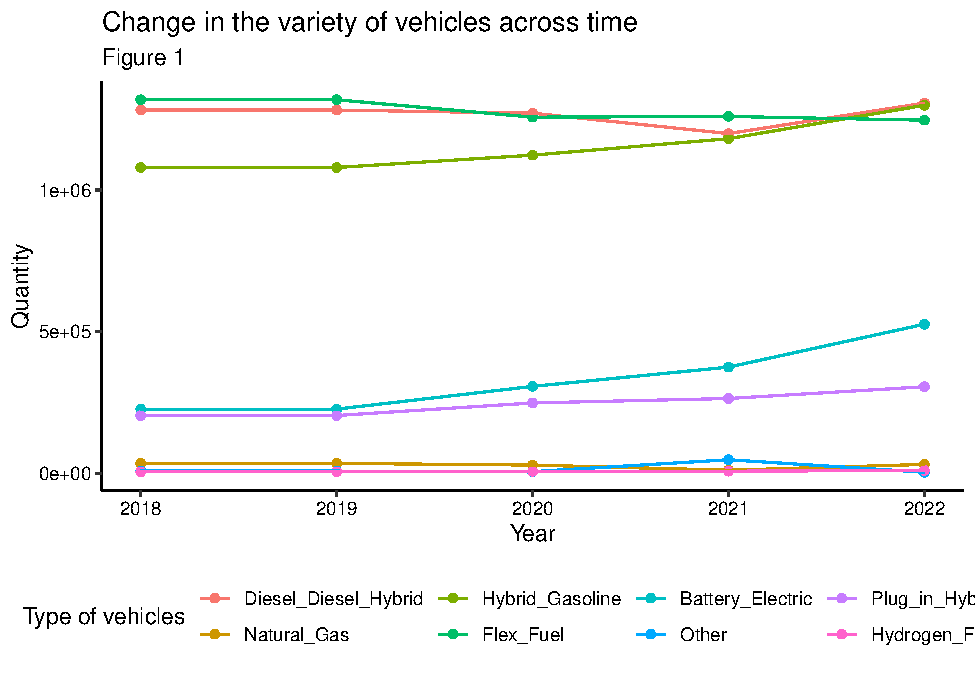
\includegraphics{Code_Main-Markdown_files/figure-latex/unnamed-chunk-3-1.pdf}
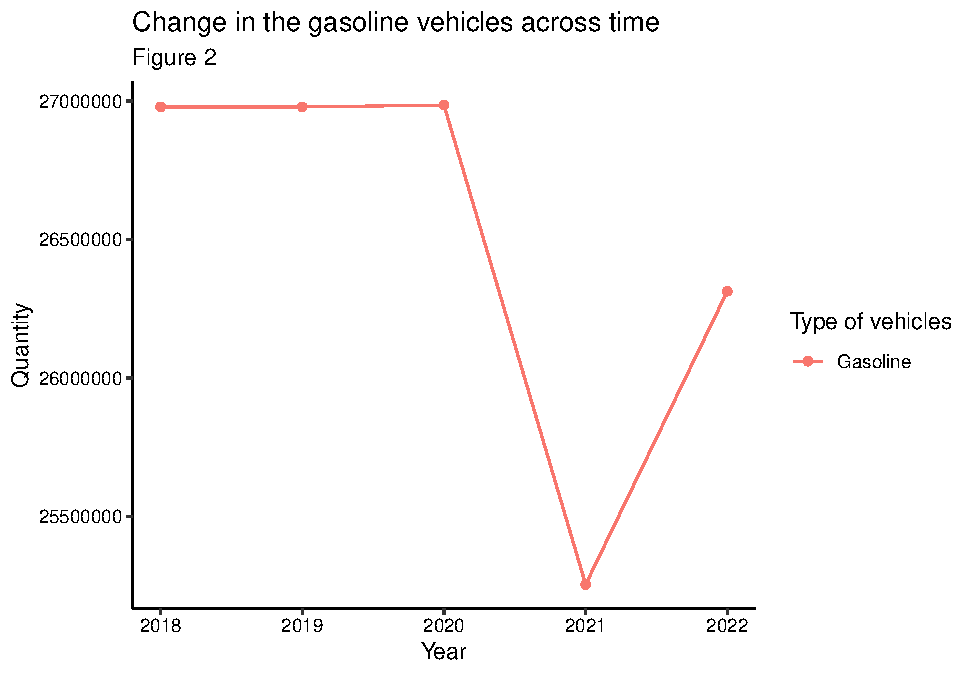
\includegraphics{Code_Main-Markdown_files/figure-latex/unnamed-chunk-3-2.pdf}

\emph{Trends of heavy and light duty cars over time}

Figure 3 below shows the trend of heavy vehicles by vehicle type across
time. The state has a higher share (more than 50 percent) of heavy-duty
gasoline and diesel-run vehicles than other types of vehicles. The
natural gas heavy-duty vehicle has shown an increase in 2020 and then a
slight decline since 2021. The share of other types of heavy-duty
vehicles such as gasoline, hybrid gasoline, and flex-fuel vehicles has
remained below 5 percent over time.

Figure 4 below shows the trend of light vehicles by vehicle type across
time. Natural gas light-duty vehicle has shown a decline in 2020 and
then a slight increase since 2021. The share of other types of
light-duty vehicles such as gasoline, hybrid gasoline, and flex-fuel
vehicles has remained higher than 90 percent over time.

Note: Share is calculated as for example, heavy-duty vehicle
diesel/Total diesel vehicles

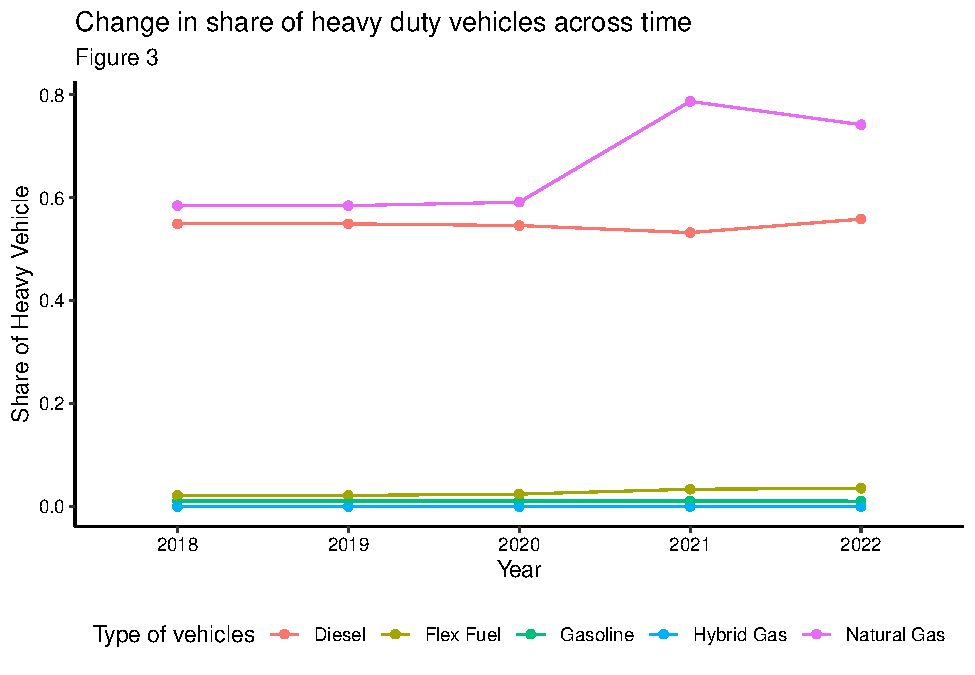
\includegraphics{Code_Main-Markdown_files/figure-latex/unnamed-chunk-4-1.pdf}
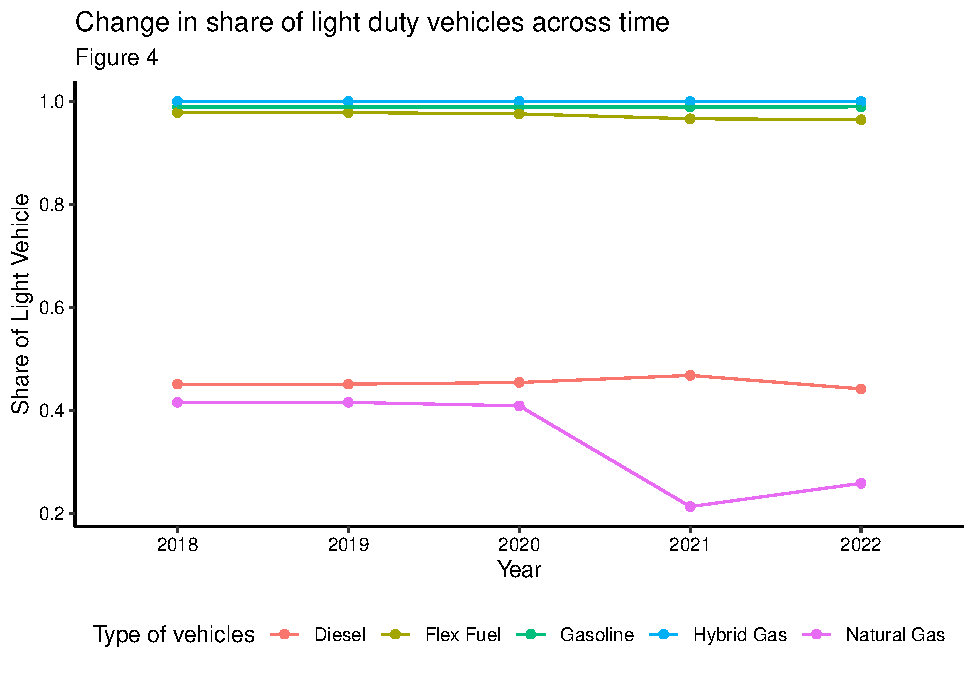
\includegraphics{Code_Main-Markdown_files/figure-latex/unnamed-chunk-4-2.pdf}

\newpage

\hypertarget{analysis}{%
\section{Analysis}\label{analysis}}

This section is divided into two types of analysis: Trend Analysis and
Regression Analysis

\hypertarget{question-1}{%
\subsection{Question 1}\label{question-1}}

What are the trends of two types of emission, nitrogen oxide and carbon
monoxide, from diesel-run, gas-run, light-duty and heavy-duty vehicles.

\emph{Comparison of nitrogen oxide and carbon monoxide emissions of
diesel-run vehicles.}

Figure 5 and 6 below shows the trend of nitrogen oxide and carbon
monoxide emissions of diesel-run vehicles over time, respectively. The
overall trend of nitrogen oxide emissions has shown a declining trend
across all the subcategories. The carbon monoxide emissions trend of
diesel-run vehicles remains like nitrogen oxide emission except for
heavy-duty diesel urban buses which has increased over time.

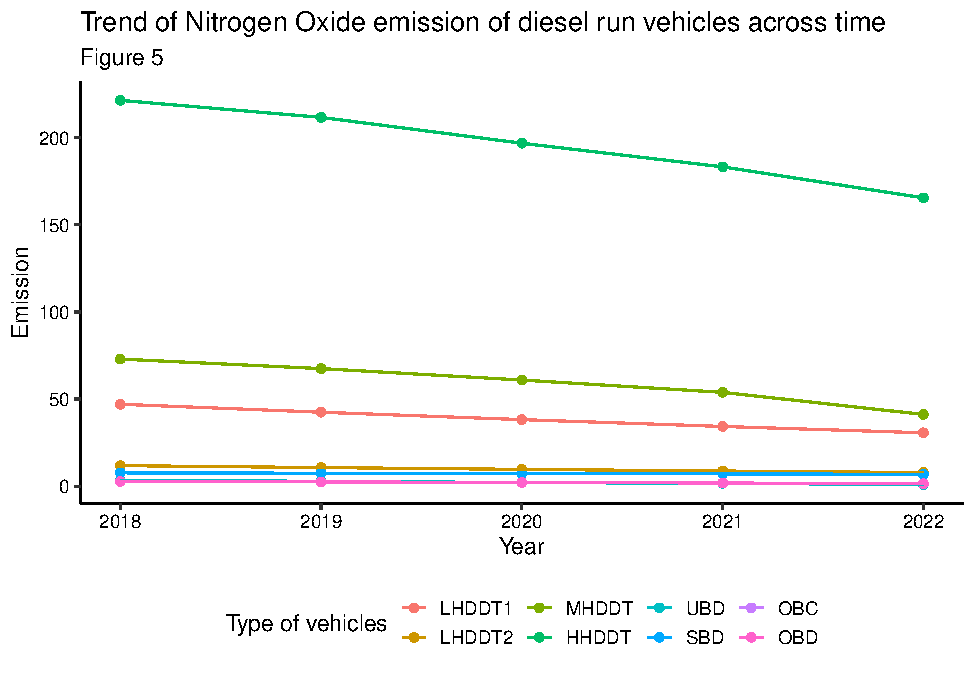
\includegraphics{Code_Main-Markdown_files/figure-latex/unnamed-chunk-5-1.pdf}
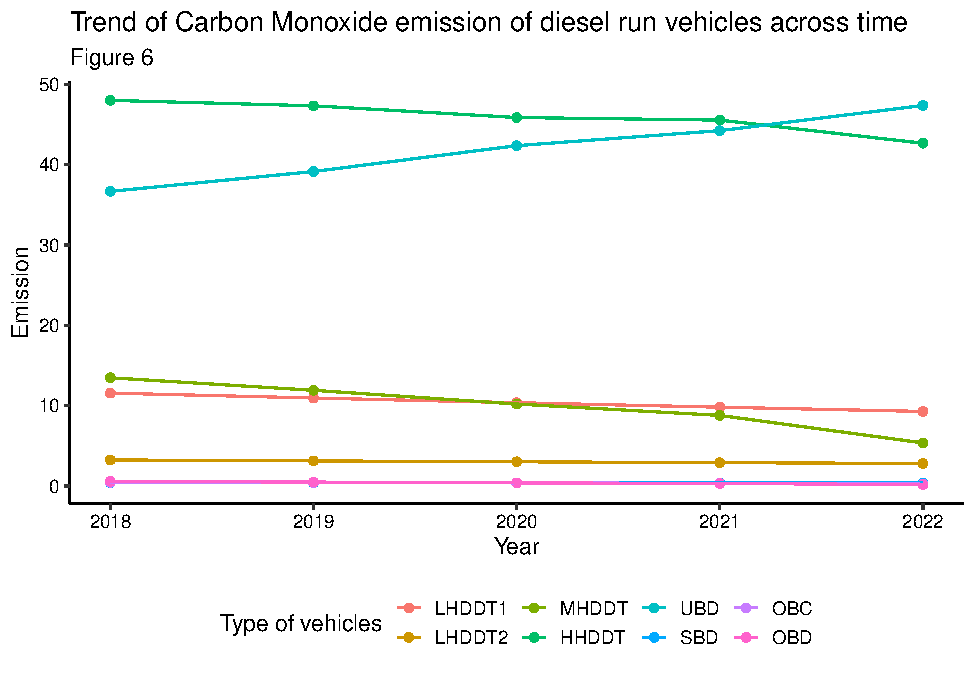
\includegraphics{Code_Main-Markdown_files/figure-latex/unnamed-chunk-5-2.pdf}

\emph{Comparison of nitrogen oxide and carbon monoxide emissions of
gas-run vehicles.}

Figure 7 and 8 below shows the trend of nitrogen oxide and carbon
monoxide emissions of gas-run vehicles over time, respectively. The
trend shows that both types of emissions from gas-run vehicles have
decreased or remained stable over time across all the subcategories.

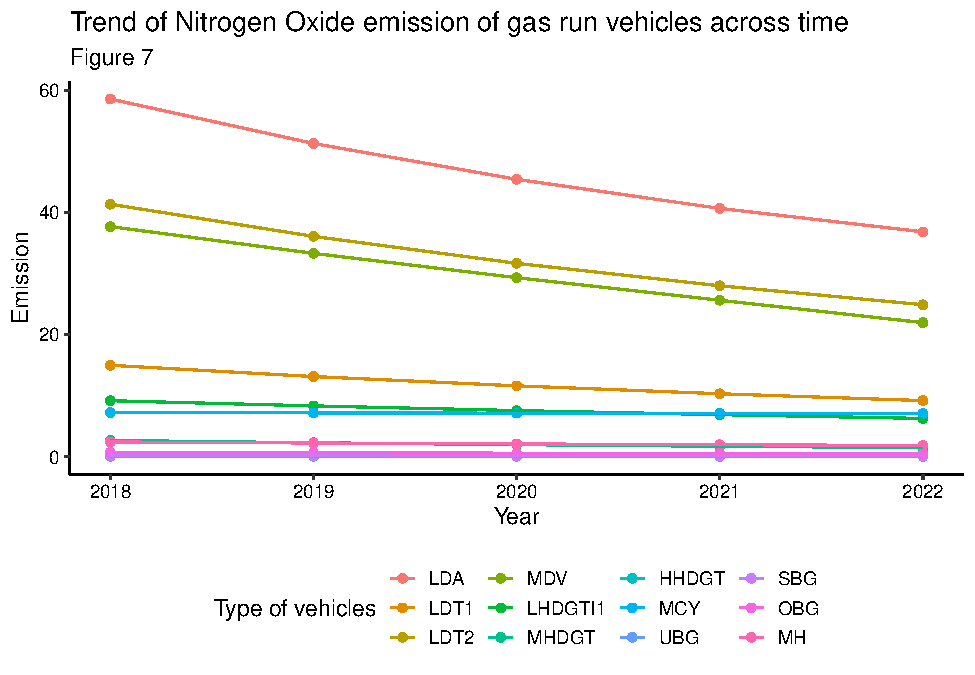
\includegraphics{Code_Main-Markdown_files/figure-latex/unnamed-chunk-6-1.pdf}
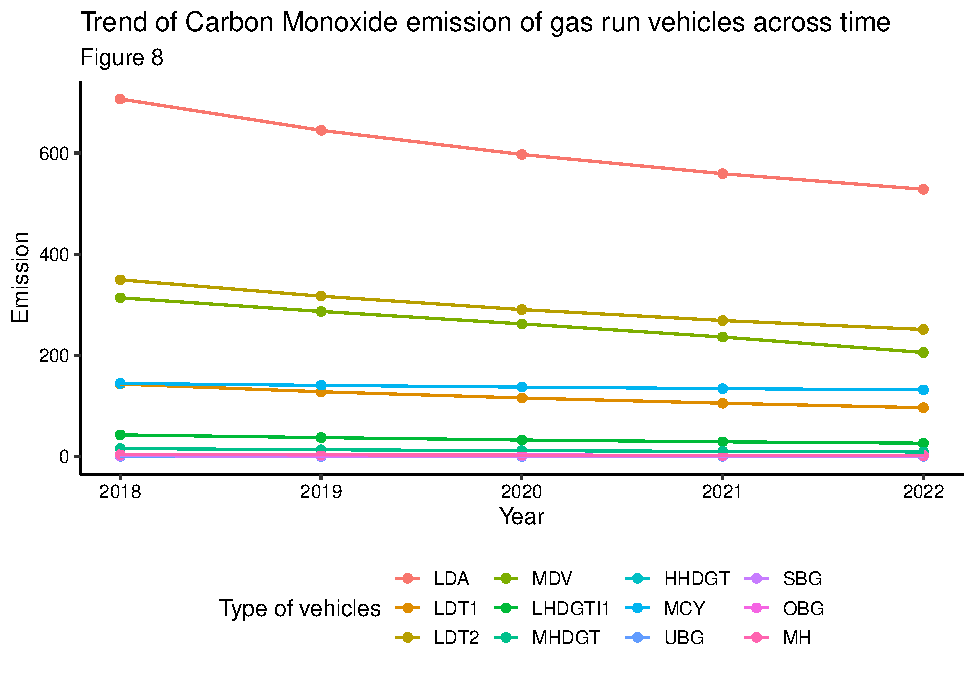
\includegraphics{Code_Main-Markdown_files/figure-latex/unnamed-chunk-6-2.pdf}

\emph{Comparison of nitrogen oxide and carbon monoxide emissions of
light-duty vehicles.}

Figure 9 and 10 below show the trend of nitrogen oxide and carbon
monoxide emissions of light-duty vehicles over time, respectively. The
trend shows that both types of emissions from light-duty vehicles have
decreased or remained stable over time across all the subcategories.

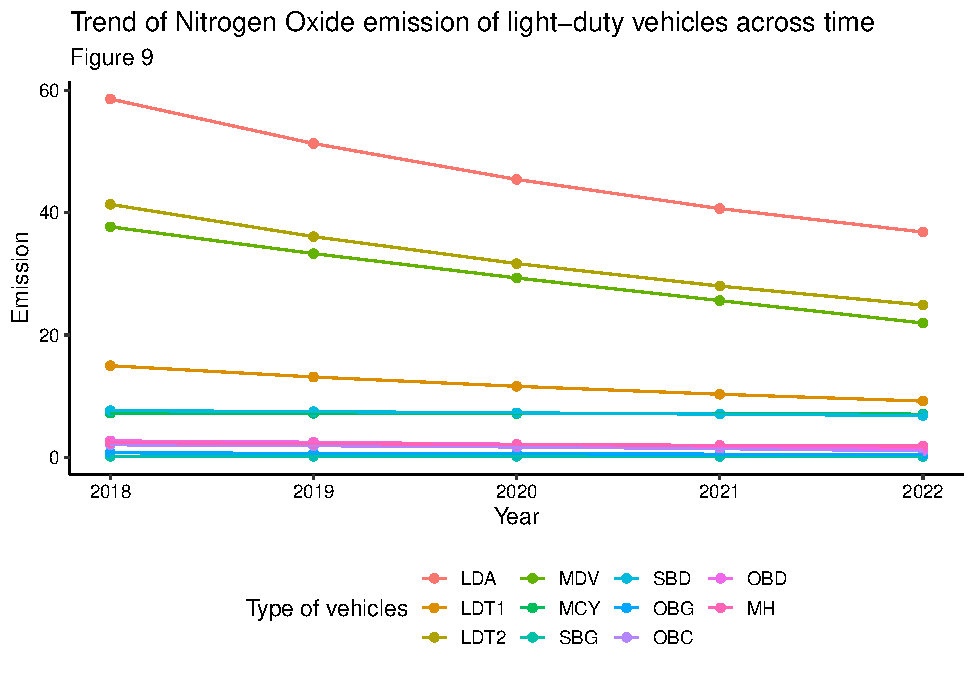
\includegraphics{Code_Main-Markdown_files/figure-latex/unnamed-chunk-7-1.pdf}
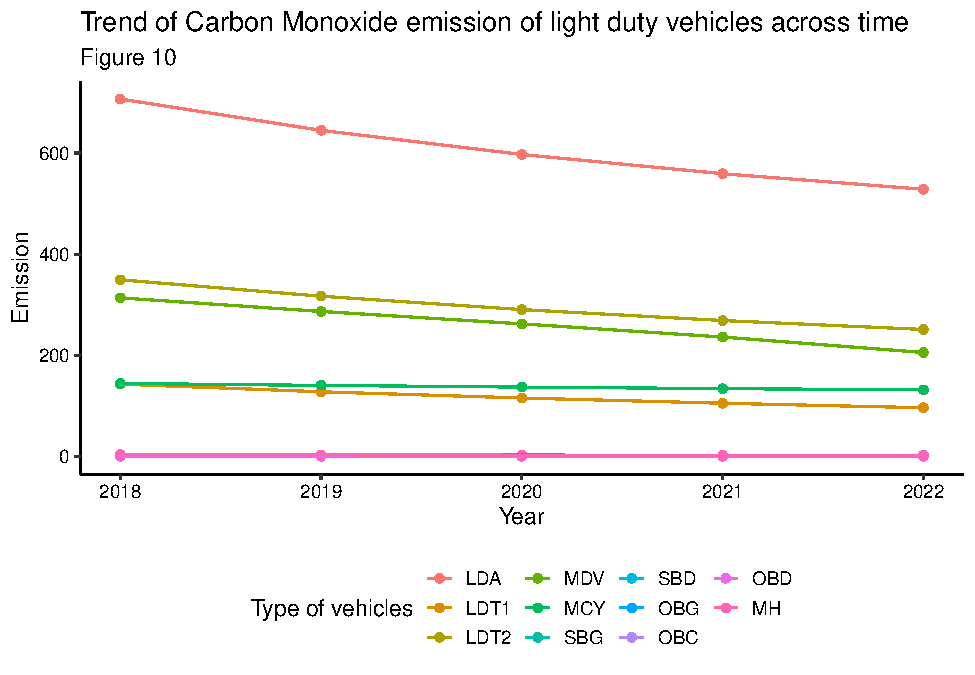
\includegraphics{Code_Main-Markdown_files/figure-latex/unnamed-chunk-7-2.pdf}

\emph{Comparison of nitrogen oxide and carbon monoxide emissions of
heavy-duty vehicles.}

Figure 11 and 12 below show the trend of nitrogen oxide and carbon
monoxide emissions of heavy-duty vehicles over time, respectively. The
trend shows that the nitrogen oxide emissions from heavy-duty vehicles
have decreased or remained stable over time across all the
subcategories. The arbon monoxide emissions trend of diesel-run vehicles
remains like nitrogen oxide emission except for heavy-duty diesel urban
buses which has increased over time.

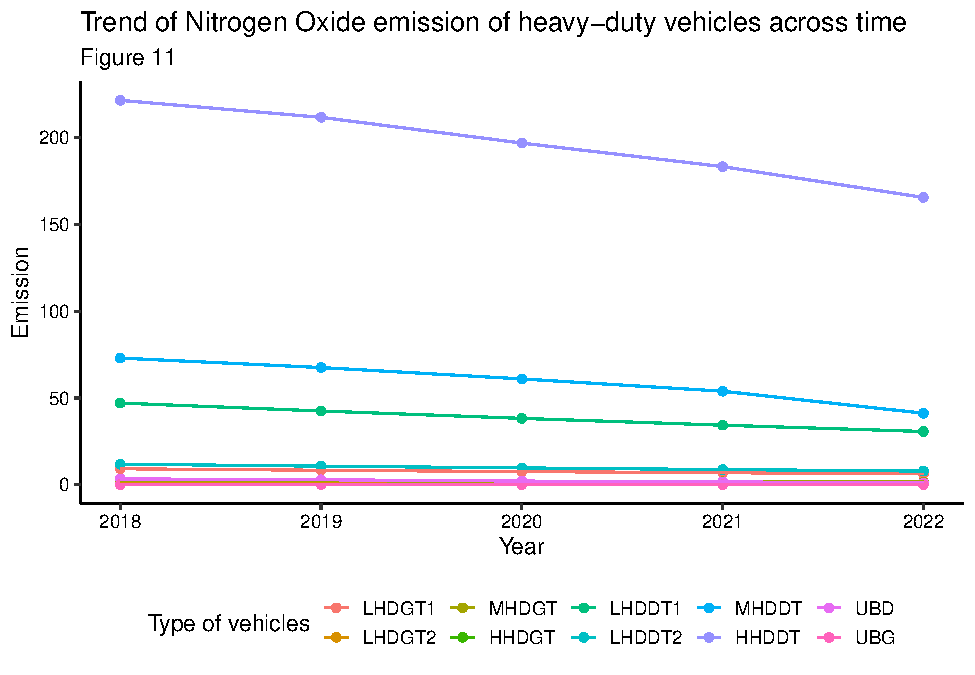
\includegraphics{Code_Main-Markdown_files/figure-latex/unnamed-chunk-8-1.pdf}
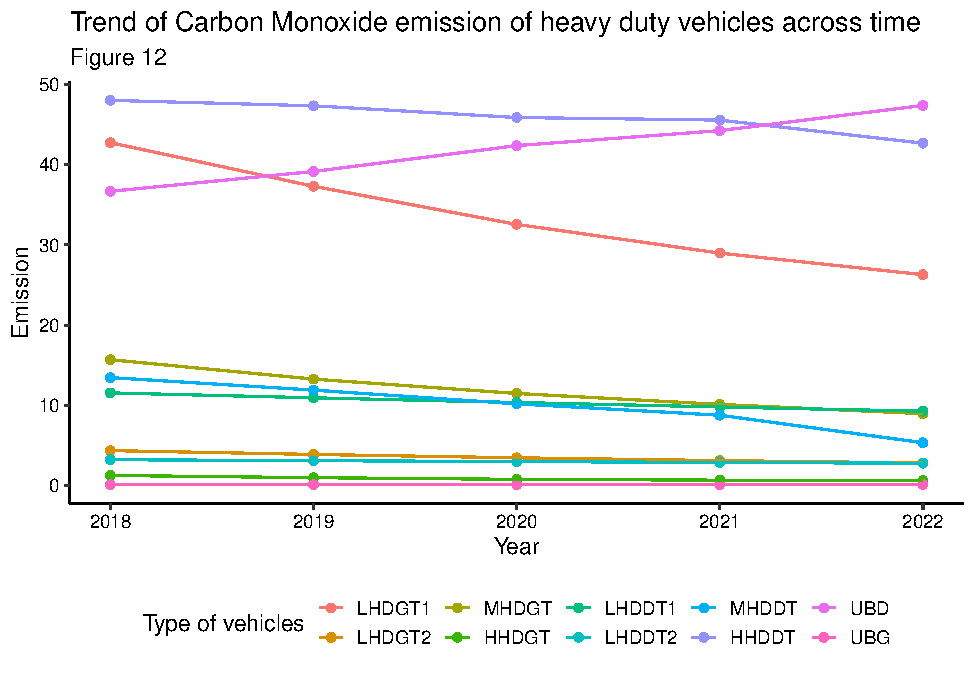
\includegraphics{Code_Main-Markdown_files/figure-latex/unnamed-chunk-8-2.pdf}

\hypertarget{question-2}{%
\subsection{Question 2}\label{question-2}}

For two kinds of pollutants (COT and NOX), how does the number of
vehicles contribute to the changes in emissions?

\hypertarget{sub-question}{%
\subsubsection{Sub question}\label{sub-question}}

Are types of fuel (diesel and gas) contribute to the emission
differently?

\begin{verbatim}
## 
## Call:
## lm(formula = Emission.diesel ~ Quantity.diesel, data = ds4)
## 
## Residuals:
##      1      2      3      4      5 
##  2.255  1.636  0.680 -1.110 -3.461 
## 
## Coefficients:
##                   Estimate Std. Error t value Pr(>|t|)  
## (Intercept)      1.321e+02  4.161e+01   3.175   0.0503 .
## Quantity.diesel -1.561e-05  3.279e-05  -0.476   0.6665  
## ---
## Signif. codes:  0 '***' 0.001 '**' 0.01 '*' 0.05 '.' 0.1 ' ' 1
## 
## Residual standard error: 2.673 on 3 degrees of freedom
## Multiple R-squared:  0.07025,    Adjusted R-squared:  -0.2397 
## F-statistic: 0.2267 on 1 and 3 DF,  p-value: 0.6665
\end{verbatim}

\begin{verbatim}
## 
## Call:
## lm(formula = ds4$Emission.gas ~ ds4$Quantity.gas)
## 
## Residuals:
##       1       2       3       4       5 
##  179.98   30.00  -93.69   72.47 -188.76 
## 
## Coefficients:
##                    Estimate Std. Error t value Pr(>|t|)
## (Intercept)      -2.678e+03  2.918e+03  -0.917    0.427
## ds4$Quantity.gas  1.567e-04  1.101e-04   1.424    0.250
## 
## Residual standard error: 166.3 on 3 degrees of freedom
## Multiple R-squared:  0.4032, Adjusted R-squared:  0.2043 
## F-statistic: 2.027 on 1 and 3 DF,  p-value: 0.2497
\end{verbatim}

We first ran a simple regression to estimate the relationship between
the number of vehicles using diesel and the emission of carbon organic
total(COT). The quantity of cars is the independent variable, and the
emission is the dependent variable in the model. The estimated effect of
the number of cars on the COT emission is --0.00001561. e p-value is
0.665, which is much larger than 0.05. We could say the quantity has no
statistically significant effect on the emission.

Then we tested the relationship between the number of gas-fueled
vehicles and the COT emission. The quantity of cars is the independent
variable, and the emission is the dependent variable in the model. The
estimated effect of the number of cars on the COT emission is 0.0001567.
Compared with the result of diesel, we could observe a slightly larger
effect. The p-value is 0.250, which is much larger than 0.05. We could
say the number of cars has no statistically significant effect on the
emission. Coefficient (absolute value) for gas is much higher than
diesel, thus gas vehicle produces more COT emission

\begin{verbatim}
## 
## Call:
## lm(formula = Emission.diesel ~ Quantity.diesel, data = ds5)
## 
## Residuals:
##       1       2       3       4       5 
##  51.056  29.198   2.108 -18.960 -63.402 
## 
## Coefficients:
##                  Estimate Std. Error t value Pr(>|t|)
## (Intercept)     2.190e+02  7.959e+02   0.275    0.801
## Quantity.diesel 7.562e-05  6.272e-04   0.121    0.912
## 
## Residual standard error: 51.13 on 3 degrees of freedom
## Multiple R-squared:  0.004823,   Adjusted R-squared:  -0.3269 
## F-statistic: 0.01454 on 1 and 3 DF,  p-value: 0.9117
\end{verbatim}

\begin{verbatim}
## 
## Call:
## lm(formula = ds5$Emission.gas ~ ds5$Quantity.gas)
## 
## Residuals:
##       1       2       3       4       5 
##  24.735   4.319 -13.059   9.967 -25.963 
## 
## Coefficients:
##                    Estimate Std. Error t value Pr(>|t|)
## (Intercept)      -4.359e+02  4.020e+02  -1.084    0.358
## ds5$Quantity.gas  2.178e-05  1.517e-05   1.436    0.247
## 
## Residual standard error: 22.91 on 3 degrees of freedom
## Multiple R-squared:  0.4073, Adjusted R-squared:  0.2098 
## F-statistic: 2.062 on 1 and 3 DF,  p-value: 0.2465
\end{verbatim}

We used another pollutant, nitrogen oxides (NOX). Similar to what we did
for NOX, we first tested the relationship between the number of
diesel-fueled vehicles and the NOX emission. The quantity of cars is the
independent variable, and the emission is the dependent variable in the
model. The estimated effect of the number of cars on the NOX emission is
0.00007562. The p-value is 0.912, which is much larger than 0.05. We
could say the number of cars has no statistically significant effect on
the emission.

Then we ran the regression to estimate the relationship between the
number of gas-fueled vehicles and the NOX emission. The quantity of cars
is the independent variable, and the emission is the dependent variable
in the model. The estimated effect of the number of cars on the NOX
emission is 0.00002178. We could see the result of diesel-fueled cars is
slightly larger than the one of gas-fueled. The p-value is 0.247, which
is much larger than 0.05. We could say the number of cars has no
statistically significant effect on the emission.

\hypertarget{question3}{%
\subsection{Question3}\label{question3}}

Is there any difference in the contribution to emission between heavy
duty urban buses fueled by gas and diesel?

\begin{verbatim}
##        2        3        4        5        6 
## 1844.808 1694.213 1570.754 1464.898 1365.674
\end{verbatim}

\begin{verbatim}
## 
## Call:
## lm(formula = Total_Emission ~ `HEAVY DUTY DIESEL URBAN BUSES (UBD)` + 
##     `HEAVY DUTY GAS URBAN BUSES (UBG)`, data = ds6)
## 
## Residuals:
##       2       3       4       5       6 
##  17.381 -19.619   9.443 -22.898  15.693 
## 
## Coefficients:
##                                        Estimate Std. Error t value Pr(>|t|)  
## (Intercept)                            3001.223   1284.956   2.336    0.145  
## `HEAVY DUTY DIESEL URBAN BUSES (UBD)`   -46.308      5.734  -8.077    0.015 *
## `HEAVY DUTY GAS URBAN BUSES (UBG)`     3933.293  10938.720   0.360    0.754  
## ---
## Signif. codes:  0 '***' 0.001 '**' 0.01 '*' 0.05 '.' 0.1 ' ' 1
## 
## Residual standard error: 27.81 on 2 degrees of freedom
## Multiple R-squared:  0.9891, Adjusted R-squared:  0.9782 
## F-statistic: 90.88 on 2 and 2 DF,  p-value: 0.01088
\end{verbatim}

Only using the COT emission data, we ran a multivariable regression to
estimate different types of heavy-duty urban buses' contribution to the
total emission. The null hypothesis is the coefficient of heavy duty
diesel urban buses and the coefficient of heavy duty gas urban buses are
the same. Regarding the heavy duty diesel urban buses, the coefficient
is -46.308 and the p-value is 0.015, which is smaller than 0.05. We
could reject the null hypothesis that the beta1 (coefficient of heavy
duty diesel urban buses) is statistically different from others. And for
the heavy duty gas urban buses, the coefficient is 3933.293 and the
p-value is 0.754, which is much larger than 0.05. From the regression
result, we could say that for the same type of heavy duty urban buses,
the fuel type (diesel and gas) has a clearly different impact on the
total emission. The limitation of the analysis is that we could not find
available data of the number of two types of urban buses.

\newpage

\hypertarget{summary-and-conclusions}{%
\section{Summary and Conclusions}\label{summary-and-conclusions}}

{[}1{]} Number of gasoline vehicle are highest followed by hybrid
gasoline, diesel run and flex fuel vehicles. Share of vehicle on natural
gas, electric battery and hydrogen fuel are the lowest. {[}2{]} More
than 50\% of vehicles running on natural gas and diesel are heavy duty
vehicles whereas, less than 5\% of gasoline, hybrid gasoline and flex
fuel vehicle are heavy duty vehicles. This share has remain stable over
time except for natural gas for which share of heavy-duty vehicle
increased since 2020. {[}3{]} Trend of nitrogen oxide emissions has
shown a declining trend across all the subcategories of vehicles. The
carbon monoxide emissions trend of diesel-run vehicles remains similar
to the trend of nitrogen oxide emission except for heavy-duty diesel
urban buses for which carbon emission has increased over time. {[}4{]}
Both types of emissions from gas-run vehicles have decreased or remained
stable over time across all the subcategories. {[}5{]} Both types of
emissions from light-duty vehicles have decreased or remained stable
over time across all the subcategories. {[}6{]} The nitrogen oxide
emissions from heavy-duty vehicles have decreased or remained stable
over time across all the subcategories. The carbon monoxide emissions
trend of diesel-run vehicles remains similar to the trend of nitrogen
oxide emission except for heavy-duty diesel urban buses for which carbon
emission has increased over time. {[}7{]} From the regression result,
for the same type of heavy duty urban buses, the fuel type (diesel and
gas) has a clearly different impact on the total emission.

\newpage

\hypertarget{reference}{%
\section{Reference}\label{reference}}

{[}1{]}``California Moves to Accelerate to 100\% New Zero-Emission
Vehicle Sales by 2035 \textbar{} California Air Resources Board,''
accessed December 13, 2022,
\url{https://ww2.arb.ca.gov/news/california-moves-accelerate-100-new-zero-emission-vehicle-sales-2035}.

{[}2{]} ``2022 Scoping Plan Documents \textbar{} California Air
Resources Board,'' accessed December 13, 2022,
\url{https://ww2.arb.ca.gov/our-work/programs/ab-32-climate-change-scoping-plan/2022-scoping-plan-documents}.

{[}3{]} ``Greenhouse Gases Emitted in California,'' accessed December
13, 2022, \url{https://datawrapper.dwcdn.net/PR9hr/7/}.

{[}4{]} Joe Robertson, ``U.S. States Ranked by Carbon Dioxide Emissions
per Capita - Solar Power Guide - Infographic,'' accessed December 13,
2022,
\url{https://solarpower.guide/solar-energy-insights/states-ranked-carbon-dioxide-emissions}.

\end{document}
